\documentclass[english,11pt,table,handout]{beamer}

% Copyright 2007 by Till Tantau
%
% This file may be distributed and/or modified
%
% 1. under the LaTeX Project Public License and/or
% 2. under the GNU Public License.
%
% See the file doc/licenses/LICENSE for more details.


% Common packages
\usepackage[utf8x]{inputenc}
\usepackage[vietnam,english]{babel}
\usepackage[utf8]{vietnam}
%\usepackage{times}
\usefonttheme[onlymath]{serif}
\usecolortheme{default}
\usepackage{booktabs}
\usepackage{mathpartir}
\usepackage{listings}
\usepackage{listingsutf8}

\usepackage{pbox}
\mprset{flushleft}
\mode<article>
{
  \usepackage{times}
  \usepackage{mathptmx}
  \usepackage[left=1.5cm,right=6cm,top=1.5cm,bottom=3cm]{geometry}
}

\usepackage{hyperref}
\usepackage{tikz}
\usetikzlibrary{arrows,backgrounds}
%\tikzstyle{mnode}=[circle, draw, fill=black, inner sep=0pt, minimum width=4pt]
\usepackage{colortbl}
%\usepackage{yfonts}
\usepackage{translator} % comment this, if not available


% Common settings for all lectures in this course

\def\lecturename{Image Processing and Computer Vision}

\title{\insertlecture}

\author{\textbf{LE Thanh Sach}}

\institute
{
  \textit{Faculty of Computer Science and Engineering}\\
  \textit{Ho Chi Minh University of Technology, VNU-HCM}
}

\subject{Lecturer \lecturename}

% Beamer version theme settings

\useoutertheme[height=0pt,width=2cm,right]{sidebar}
\usecolortheme{rose,sidebartab}
\useinnertheme{circles}
\usefonttheme[only large]{structurebold}

\setbeamercolor{sidebar right}{bg=black!15}
\setbeamercolor{structure}{fg=blue}
\setbeamercolor{author}{parent=structure}

\setbeamerfont{title}{series=\normalfont,size=\LARGE}
\setbeamerfont{title in sidebar}{series=\bfseries}
\setbeamerfont{author in sidebar}{series=\bfseries}
\setbeamerfont*{item}{series=}
\setbeamerfont{frametitle}{size=}
\setbeamerfont{block title}{size=\small}
\setbeamerfont{subtitle}{size=\normalsize,series=\normalfont}

\setbeamertemplate{navigation symbols}{}
\setbeamertemplate{bibliography item}[book]
\setbeamertemplate{sidebar right}
{
  {\usebeamerfont{title in sidebar}%
    \vskip1.5em%
    \hskip3pt%
    \usebeamercolor[fg]{title in sidebar}%
    \insertshorttitle[width=2cm,center,respectlinebreaks]\par%
    \vskip1.25em%
  }%
  {%
    \hskip3pt%
    \usebeamercolor[fg]{author in sidebar}%
    \usebeamerfont{author in sidebar}%
    \insertshortauthor[width=2cm,center,respectlinebreaks]\par%
    \vskip1.25em%
  }%
  \hbox to2cm{\hss\insertlogo\hss}
  \vskip1.25em%
  \insertverticalnavigation{2cm}%
  \vfill
  \hbox to 2cm{\hfill\usebeamerfont{subsection in
      sidebar}\strut\usebeamercolor[fg]{subsection in
      sidebar}\insertshortlecture.\insertframenumber\hskip5pt}%
  \vskip3pt%
}%

\setbeamertemplate{title page}
{
  \vbox{}
  \vskip1em
  {\huge Chapter \insertshortlecture\par}
  {\usebeamercolor[fg]{title}\usebeamerfont{title}\inserttitle\par}%
  \ifx\insertsubtitle\@empty%
  \else%
    \vskip0.25em%
    {\usebeamerfont{subtitle}\usebeamercolor[fg]{subtitle}\insertsubtitle\par}%
  \fi%     
  \vskip1em\par
  \emph{\lecturename}\ 
  %on \insertdate\par
  \vskip3em\par

  \leftskip=0pt plus1fill\insertauthor\par
  \insertinstitute\vskip1em
}

\logo{
\includegraphics[width=1.5cm]{hcmut.png}}



% Article version layout settings

\mode<article>

\makeatletter
\def\@listI{\leftmargin\leftmargini
  \parsep 0pt
  \topsep 5\p@   \@plus3\p@ \@minus5\p@
  \itemsep0pt}
\let\@listi=\@listI


\setbeamertemplate{frametitle}{\paragraph*{\insertframetitle\
    \ \small\insertframesubtitle}\ \par
}
\setbeamertemplate{frame end}{%
  \marginpar{\scriptsize\hbox to 1cm{\sffamily%
      \hfill\strut\insertshortlecture.\insertframenumber}\hrule height .2pt}}
\setlength{\marginparwidth}{1cm}
\setlength{\marginparsep}{4.5cm}

\def\@maketitle{\makechapter}

\def\makechapter{
  \newpage
  \null
  \vskip 2em%
  {%
    \parindent=0pt
    \raggedright
    \sffamily
    \vskip8pt
    {\fontsize{36pt}{36pt}\selectfont Chapter \insertshortlecture \par\vskip2pt}
    {\fontsize{24pt}{28pt}\selectfont \color{blue!50!black} \insertlecture\par\vskip4pt}
    {\Large\selectfont \color{blue!50!black} \insertsubtitle\par}
    \vskip10pt

    \normalsize\selectfont Print version of
    Lecturer \emph{\lecturename} of \@date\par\vskip1.5em
    %\hfill Le Thanh Sach and Luong The Nhan, Faculty of CSE, HCMC University of Technology
  }
  \par
  \vskip 1.5em%
}

\let\origstartsection=\@startsection
\def\@startsection#1#2#3#4#5#6{%
  \origstartsection{#1}{#2}{#3}{#4}{#5}{#6\normalfont\sffamily\color{blue!50!black}\selectfont}}

\makeatother

\mode
<all>




% Typesetting Listings

\usepackage{listings}
\lstset{language=Java}

\alt<presentation>
{\lstset{%
  basicstyle=\footnotesize\ttfamily,
  commentstyle=\slshape\color{green!50!black},
  keywordstyle=\bfseries\color{blue!50!black},
  identifierstyle=\color{blue},
  stringstyle=\color{orange},
  escapechar=\#,
  emphstyle=\color{red}}
}
{
  \lstset{%
    basicstyle=\ttfamily,
    keywordstyle=\bfseries,
    commentstyle=\itshape,
    escapechar=\#,
    emphstyle=\bfseries\color{red}
  }
}



% Common theorem-like environments

\theoremstyle{example}
\newtheorem{exercise}[theorem]{\translate{Exercise}}


% New useful definitions:

\newbox\mytempbox
\newdimen\mytempdimen

\newcommand\includegraphicscopyright[3][]{%
  \leavevmode\vbox{\vskip3pt\raggedright\setbox\mytempbox=\hbox{\includegraphics[#1]{#2}}%
    \mytempdimen=\wd\mytempbox\box\mytempbox\par\vskip1pt%
    \fontsize{3}{3.5}\selectfont{\color{black!25}{\vbox{\hsize=\mytempdimen#3}}}\vskip3pt%
}}

\newenvironment{colortabular}[1]{\medskip\rowcolors[]{1}{blue!20}{blue!10}\tabular{#1}\rowcolor{blue!40}}{\endtabular\medskip}

\def\equad{\leavevmode\hbox{}\quad}

\newenvironment{greencolortabular}[1]
{\medskip\rowcolors[]{1}{green!50!black!20}{green!50!black!10}%
  \tabular{#1}\rowcolor{green!50!black!40}}%
{\endtabular\medskip}
\usepackage{pgf}

\newcommand{\Rule}[2]{\genfrac{}{}{0.7pt}{}{{\setlength{\fboxrule}{0pt}\setlength{\fboxsep}{3mm}\fbox{$#1$}}}{{\setlength{\fboxrule}{0pt}\setlength{\fboxsep}{3mm}\fbox{$#2$}}}}

\newcommand{\Rulee}[3]{\genfrac{}{}{0.7pt}{}{{\setlength{\fboxrule}{0pt}\setlength{\fboxsep}{3mm}\fbox{$#1$}}}{{\setlength{\fboxrule}{0pt}\setlength{\fboxsep}{3mm}\fbox{$#2$}}}[#3]}

\usepackage{url}

\usepackage{qtree}

\usepackage{datetime}

\usepackage{amsfonts}
\usepackage{mathtools}
\usepackage{fancybox}
\usepackage[linesnumbered]{algorithm2e}
\usepackage{ragged2e}

\lecture[7.1]{Edge Detection}{lecture-text}

% \subtitle{Sequence Control}

\date{09 September 2015}
\newcounter{saveenumi}

\usepackage{wrapfig}
\usetikzlibrary{automata,arrows,positioning, chains, shapes.callouts, calc}

\tikzstyle{mnode}=[circle, draw, fill=black, inner sep=0pt, minimum width=4pt]
\tikzstyle{thinking} = [draw=blue, very thick]
\edef\sizetape{1cm}
\tikzstyle{tmtape}=[draw,minimum size=\sizetape]
\tikzstyle{tmhead}=[arrow box,draw,minimum size=.5cm,arrow box
arrows={east:.25cm, west:0.25cm}]
\tikzset{
  level/.style   = { ultra thick, blue },
  connect/.style = { dashed, red },
  notice/.style  = { draw, rectangle callout, callout relative pointer={#1} },
  label/.style   = { text width=4cm }
}

\begin{document}

\begin{frame}
\selectlanguage{english}
  \maketitle
\end{frame}

\begin{frame}\frametitle<presentation>{Overview}
  \tableofcontents
\end{frame}

%%%%%%%%%%%%%%%%%%%%%%%%%%%%%%%%%%%%%%%%%%%%%%%%%%%%%%%%%%%%%%%%%%%%%
%%%%%%%%%%%%%%%%%%%%%%%%%%%%%%%%%%%%%%%%%%%%%%%%%%%%%%%%%%%%%%%%%%%%%

\section{Point Detection}
\frame
{
	\frametitle{Point Detection}
	\begin{enumerate}
		\item Filter the input image $f(x,y)$ with Laplacian $H_{lap}$, i.e., compute $g(x,y) = f(x,y)*H_{lap}(i,j)$
		\item Detect isolated points $(x,y)$ if they satisfy: $|g(x,y)| \ge T$. Where, $T$ is a threshold value.
	\end{enumerate}
	
	Laplacian kernel $H_{lap}$:
	
	\centering
	$$
	H_{lap} = \left[
	\begin{array}{rrr}
		-1 & -1 & -1 \\ 
		-1 & 8 & -1 \\
		-1 & -1 & -1 \\
	\end{array}
	\right]
	$$

}
\section{Line Detection}
\frame
{
	\frametitle{Line Detection}
	\begin{enumerate}
		\item Filter the input image $f(x,y)$ with all following masks for detecting horizontal, vertical, $\pm 45^0$-oriented lines. This process results $g_{i}(x,y), i=1..4$. You can design new masks for other lines with new orientation.
		\item Chose a orientation $i$ for point $(x,y)$ by selecting the largest $g_{i}(x,y), i=1..4$.
		\item Do thresholding with a certain $T$ (input) to obtain lines.
	\end{enumerate}
	
	Some kernels:

	\centering
	
	\begin{tabular}{c|c}
		$
		\left[
		\begin{array}{rrr}
		-1 & -1 & -1 \\ 
		2 & 2 & 2 \\
		-1 & -1 & -1 \\
		\end{array}
		\right]
		$ &
		$
		\left[
		\begin{array}{rrr}
		-1 & 2 & -1 \\ 
		-1 & 2 & -1 \\
		-1 & 2 & -1 \\
		\end{array}
		\right]
		$
		\\
		Horizontal & Vertical 
		\\
		\hline
		$
		\left[
		\begin{array}{rrr}
		-1 & -1 & 2 \\ 
		-1 & 2 & -1 \\
		2 & -1 & -1 \\
		\end{array}
		\right]
		$ &
		$
		\left[
		\begin{array}{rrr}
		2 & -1 & -1 \\ 
		-1 & 2 & -1 \\
		-1 & -1 & 2 \\
		\end{array}
		\right]
		$ 
		\\
		$+45^0$ & $-45^0$ 
		\\
		
	\end{tabular}
}
\section{Edge Detection}
\frame{
	\frametitle{Edge Detection}
	\selectlanguage{english}
	
	\begin{alertblock}{Definition}
		Edge is a set of connected pixels that lie on the boundary between two regions.
	\end{alertblock}
	\begin{block}{Properties}
		\begin{enumerate}
			\item There is "meaningful" transitions in gray-levels at edge.
			\item So, first-order and second-order derivatives can be used to detect the transition.
		\end{enumerate}
	\end{block}
	
}
\frame{
	\frametitle{Edge Detection}
	\selectlanguage{english}
	Examples of Derivatives: image, a line profile, first and second-order derivatives.
	
	\begin{figure}[!h]
		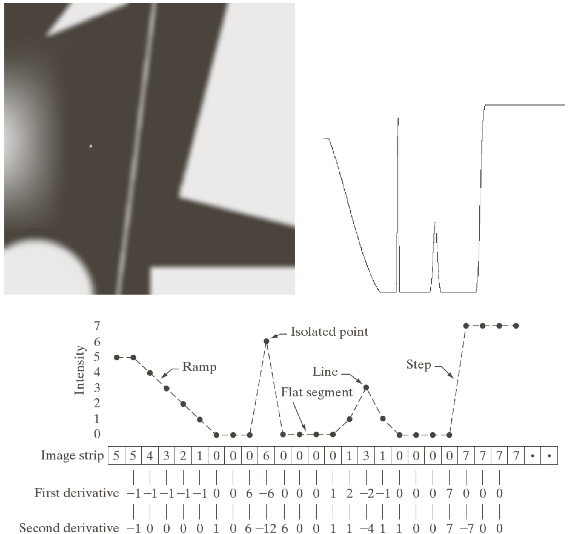
\includegraphics[height=7.5cm]{edge_derivative.png}
	\end{figure}
}


\frame{
	\frametitle{Edge Detection}
	\selectlanguage{english}
	Model of edges:
	
	\begin{figure}[!h]
		
\includegraphics[width=9cm]{edge_model.png}
	\end{figure}
	\begin{enumerate}
		\item Left: \alert{\textbf{Clear edge or Ideal edge}}, ideally represented as a step
		\item Middle: \alert{\textbf{Blurred edge}}, ideally represented as a ramp
		\item Right: \alert{\textbf{A blurred bright edge}}, ideally represented as a roof.
	\end{enumerate}
}

\frame{
	\frametitle{Edge Detection}
	\selectlanguage{english}
	
	\begin{figure}[!h]
		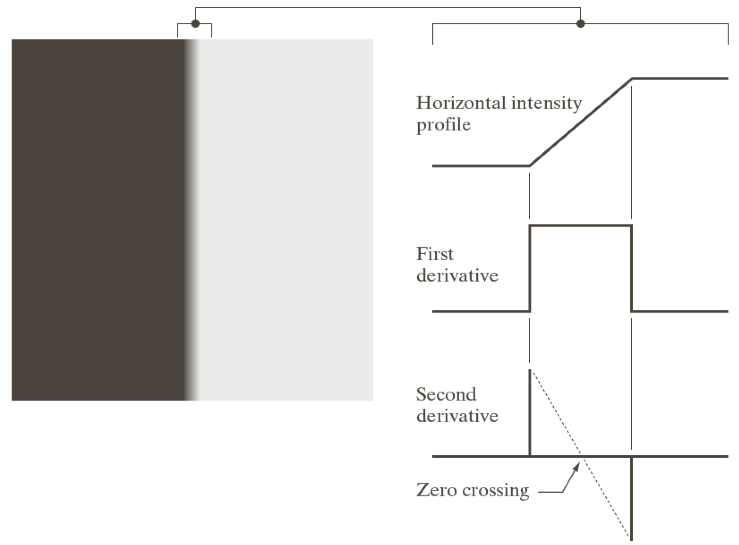
\includegraphics[height=5cm]{edge_1st_2nd.png}
	\end{figure}
	\begin{block}{Edge with first-order derivatives}
		Edge consists of points where the module of the gradient vector is greater than a threshold.
		\begin{itemize}
			\item The gradient vector is \alert{\textbf{perpendicular}} with the local edge passing that point
		\end{itemize}
	\end{block}
}
\frame{
	\frametitle{Edge Detection}
	\selectlanguage{english}
	
	\begin{figure}[!h]
		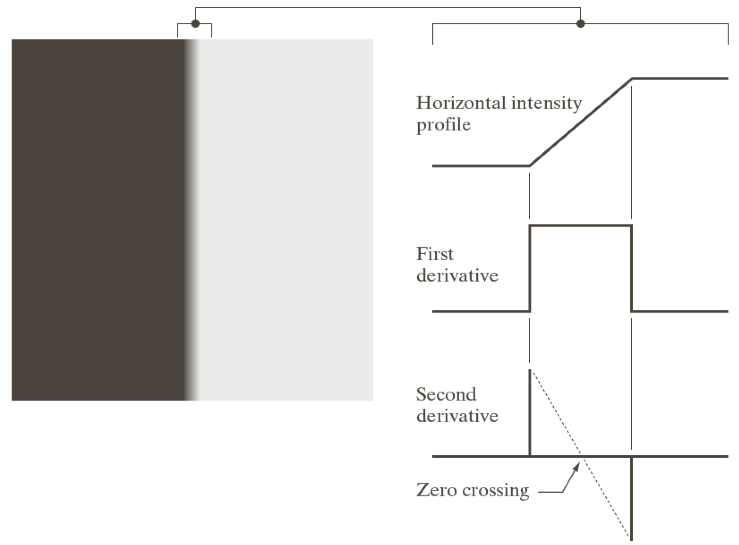
\includegraphics[height=5cm]{edge_1st_2nd.png}
	\end{figure}
	\begin{block}{Edge with second-order derivatives}
		Edge consists of \alert{\textbf{zero-crossing points}} in image filtered with second-order derivatives.
		\begin{itemize}
			\item Second-order derivatives create one \alert{\textbf{positive}} response and another \alert{\textbf{negative}} one for ramp edges.
		\end{itemize}
	\end{block}
}
\frame{
	\frametitle{Edge Detection with noise}
	\selectlanguage{english}
	
	\begin{figure}[!h]
		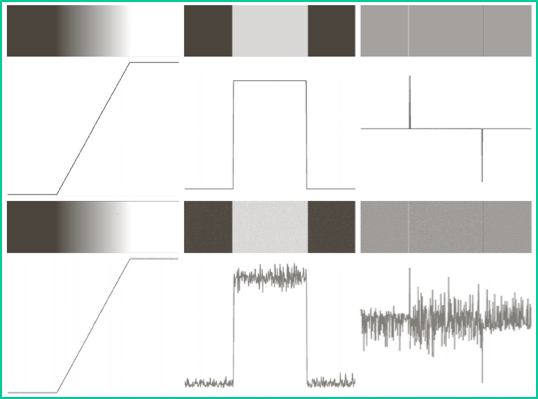
\includegraphics[height=5cm]{edge_noise_1.png}
	\end{figure}
	\begin{itemize}
		\item Rows: Row 1: no noise; Row 2: with Gaussian noise ($\mu=0, \sigma=0$)
		\item Cols: Col 1: a line profile; Col 2: \alert{\textbf{Fist-order derivative}}; Col 3: \alert{\textbf{Second-order derivative}}
	\end{itemize}
}
\frame{
	\frametitle{Edge Detection with noise}
	\selectlanguage{english}
	
	\begin{figure}[!h]
		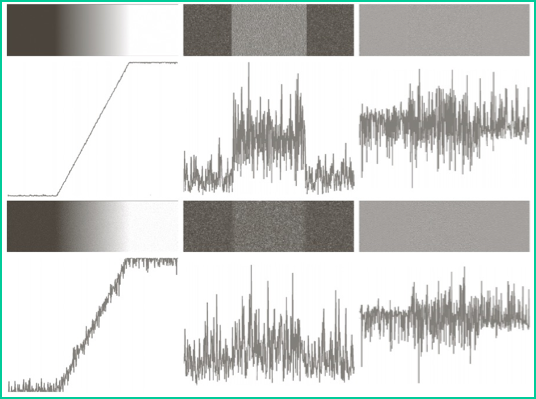
\includegraphics[height=5cm]{edge_noise_2.png}
	\end{figure}
	\begin{itemize}
		\item Rows: Row 1: with Gaussian noise ($\mu=0, \sigma=0.1$); Row 2: with Gaussian noise ($\mu=0, \sigma=1.0$)
		\item Cols: Col 1: a line profile; Col 2: \alert{\textbf{Fist-order derivative}}; Col 3: \alert{\textbf{Second-order derivative}}
	\end{itemize}
}
\frame{
	\frametitle{Edge Detection with noise}
	\selectlanguage{english}
	
	\begin{block}{Properties}
	
	\end{block}
		\begin{itemize}
			\item Second-order derivative is more \alert{\textbf{sensitive to noise}} compared with first-order derivative.
			\item However,
			\begin{itemize}
				\item First-order derivatives provide \alert{\textbf{thick edges}}
				\item Second-order derivatives provide \alert{\textbf{thin edges}} (via, zero-crossing)
			\end{itemize}
		\end{itemize}
	
}
\frame{
	\frametitle{Edge Detection and Laplacian}
	\selectlanguage{english}
	
	\begin{alertblock}{Question}
		Laplacian can provide the discontinuity in gray-levels. \alert{\textbf{Why is it not used in edge detection? }}
	\end{alertblock}
	
	\begin{block}{Reasons}
		\begin{enumerate}
			\item As a second-order derivative, it is unacceptably sensitive to noise
			\item The magnitude of Laplacian provides double edges (one for positive and another one for negative response)
			\item Laplacian can not provide edge direction
		\end{enumerate}
		 
	\end{block}
	Therefore, Laplacian is directly suitable for sharpening images only.
	
}
\frame{
	\frametitle{Edge Detection and Laplacian}
	\selectlanguage{english}
	\begin{itemize}
		\item Laplacian can provide thin edges via zeros-crossing detection. However, it is sensitive to noise. 
		\item What will be happened if we remove noise before taking Laplician and then finding zeros-crossing?
	\end{itemize}
	
	
	\begin{alertblock}{Laplacian in edge detection}
		\begin{enumerate}
			\item Perform noise removal will a Gaussian low-pass filter. The input image will be blurred.
			\item Apply Laplacian to the resulting image.
			\item Detect zero-crossing points to obtain edge points.
		\end{enumerate}
	\end{alertblock}
	\begin{block}{Laplacian of Gaussian (LoG)}
		\alert{\textbf{Step $1$ and $2$ in the above algorithm is equivalent to filtering image with a LoG mask}}
	\end{block}
	

}
\section{Laplacian of Gaussian (LoG)}
\frame{
	\frametitle{Laplacian of Gaussian (LoG)}
	\selectlanguage{english}
	
	\begin{alertblock}{A Gaussian function $G(x,y)$}
		\begin{align}
		\nonumber
			G(x,y) &= e^{-\frac{x^2 + y^2}{2\sigma^2}}
		\end{align}
	\end{alertblock}
	
	\begin{itemize}
		\item $\sigma$ : standard deviation. \alert{\textbf{This parameter decides the degree of blurring in output image, if the input image is convoluted with this function}}
	\end{itemize}	
}
\frame{
	\frametitle{Laplacian of Gaussian (LoG)}
	\selectlanguage{english}
	
	\begin{alertblock}{Laplacian of Gaussian (LoG)}
		\begin{align}
		\nonumber
		\nabla^2G(r) &= \left[ \frac{x^2 + y^2 - 2\sigma^2}{\sigma^4}\right] e^{-\dfrac{r^2}{2\sigma^2}}
		\end{align}
		\begin{itemize}
			\item LoG $\equiv$  Laplacian of function $G(x,y)$
			\item LoG $\equiv$  $\frac{\partial^2G(x,y)}{\partial x^2} + \frac{\partial^2G(x,y)}{\partial y^2}$
		\end{itemize}	
	\end{alertblock}
	
}
\frame{
	\frametitle{Laplacian of Gaussian (LoG)}
	\selectlanguage{english}
	\begin{figure}[!h]
		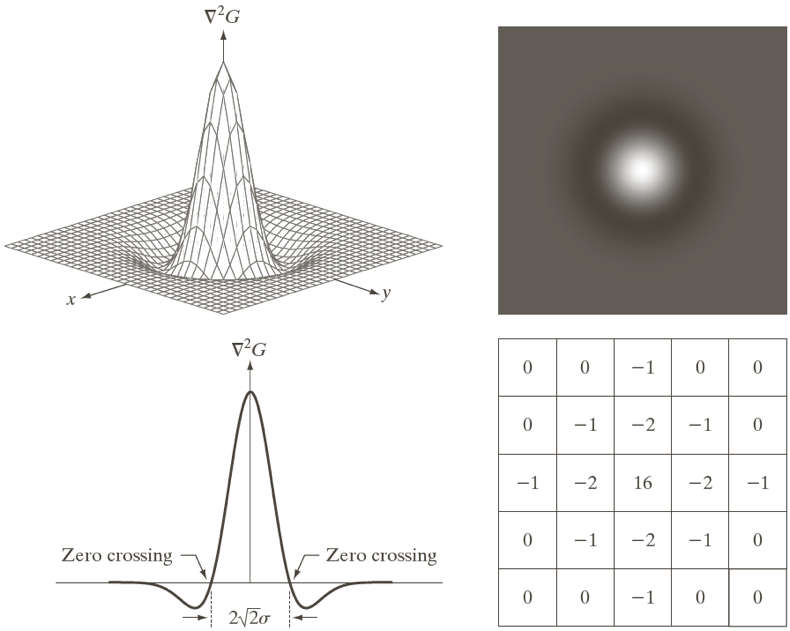
\includegraphics[height=8cm]{log.png}
	\end{figure}

}

\frame{
	\frametitle{Laplacian of Gaussian (LoG)}
	\selectlanguage{english}
	\begin{block}{Properties}
		\begin{enumerate}
			\item Other name: Mexican hat, because of its shape
			\item Zero-crossing point in LoG: $x^2 + y^2 = 2\sigma^2$
			\item Radius from the origin to zero-crossing point: $r = \sqrt{2} \sigma$
			\item Kernel of LoG given above: just an example. It can be approximated by any size and any coefficients.
			\item \alert{\textbf{Sum of all coefficients of the kernel must be $0$}}
		\end{enumerate}
	\end{block}
	\begin{alertblock}{Generation of LoG's kernel}
		How can you generate LoG's kernel?
	\end{alertblock}
	
}
\frame{
	\frametitle{Laplacian of Gaussian (LoG)}
	\selectlanguage{english}
	\begin{block}{Properties: Linearity}
		\begin{align}
			\nonumber
			g(x,y) &= \left[\nabla^2G(x,y)\right]*f(x,y)\\
			\nonumber
				&= \nabla^2 \left[G(x,y)*f(x,y)\right]
		\end{align}
	\end{block}

}
\frame{
	\frametitle{Marr-Hildreth Algorithm}
	\selectlanguage{english}
	\begin{block}{Marr-Hildreth Algorithm}
		\begin{enumerate}
			\item \alert{\textbf{Filter}} the input image $f(x,y)$ with Gaussian low-pass filter by kernel size $n \times n$ to obtain the output $g(x,y)$.
			\item \alert{\textbf{Compute}} Laplacian of $g(x,y)$ to obtain $g_L(x,y)$
			\item \alert{\textbf{Find}} zero-crossing points in $g_L(x,y)$
		\end{enumerate}
	\end{block}
	\begin{alertblock}{LoG}
		Step $1$ and $2$ can be implemented as applying LoG on the input image.
	\end{alertblock}
	
}
\frame{
	\frametitle{Marr-Hildreth Algorithm}
	\selectlanguage{english}
	\begin{alertblock}{Power of Marr-Hildreth Algorithm}
		Marr-Hildreth Algorithm can remedy the following problems in edge detection:
		\begin{enumerate}
			\item Intensity changes are not independent of image scale $\Rightarrow$  use different kernel' size.
			\item Edges are sensitive to noise, especially true for second-order derivative $\Rightarrow$  use Gaussian low-pass filter
		\end{enumerate}
	\end{alertblock}
	\begin{block}{Questions}
		\begin{enumerate}
			\item How can you obtain the kernel's size?
			\item How can you detect zero-crossing points?
		\end{enumerate}
	\end{block}
	
}
\frame{
	\frametitle{Marr-Hildreth Algorithm}
	\selectlanguage{english}
	
	\begin{alertblock}{How can you obtain the kernel's size?}
		\begin{itemize}
			\item Volume of a Gaussian function inside of circle $radius = 3\sigma$ is $99.7\%$
			\item $\Rightarrow$ Kernel size $n \times n$, where $n$ an odd numer $\ge 6\sigma$
		\end{itemize}
	\end{alertblock}
}

\frame{
	\frametitle{Marr-Hildreth Algorithm}
	\selectlanguage{english}
	
	\begin{alertblock}{How can you detect zero-crossing points?}
		\begin{enumerate}
			\item Perform thresholding of the magnitude of LoG image, i.e. $|g_l(x,y)|$, with a value $T$. 
			
			$g_l(x,y) = 
			\begin{cases}
				-1 & \text{if } (g_l(x,y) < 0) \text{ and } |g_l(x,y)| > T \\
				1 & \text{if } (g_l(x,y) > 0) \text{ and } |g_l(x,y)| > T \\
				0 & \text{ortherwise} 
			\end{cases}
			$
			\item Apply a mask $3 \times 3$ at each pixel on $g_l(x,y)$.
			\begin{tabular}{|c|c|c|}
				\hline
				NW & N & NE\\
				\hline
				W & C & E\\
				\hline
				SW & S & SE\\
				\hline
			\end{tabular}
			\item  Detect the difference on the sign at opposing corners, i.e., (W, E), (N, S), (NW, SE), and (SW, NE).
			\item If any pair of corners results a difference on the sign, then $g_l(x,y)$ is an edge point.
		\end{enumerate}
	\end{alertblock}
}
\frame{
	\frametitle{Laplacian of Gaussian (LoG): Illustration}
	\selectlanguage{english}
	\begin{figure}[!h]
		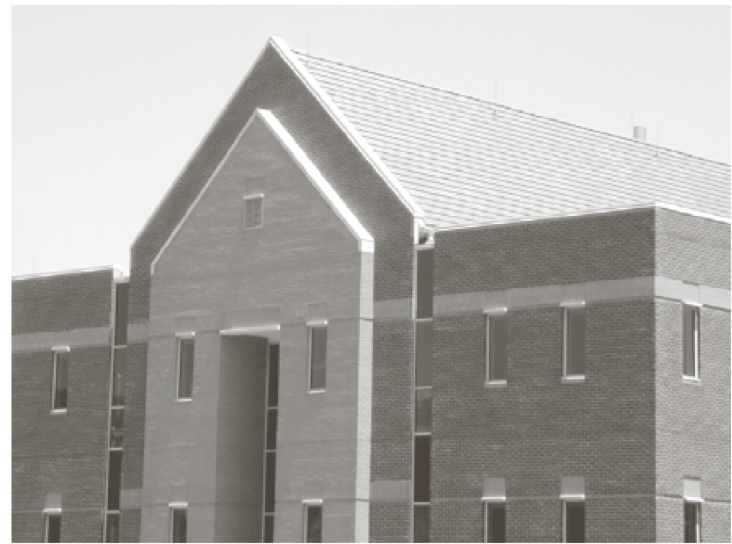
\includegraphics[height=7cm]{log_edge_original.png}
		\caption{Original image}
	\end{figure}
	
}


\frame{
	\frametitle{Laplacian of Gaussian (LoG): Illustration}
	\selectlanguage{english}
	\begin{figure}[!h]
		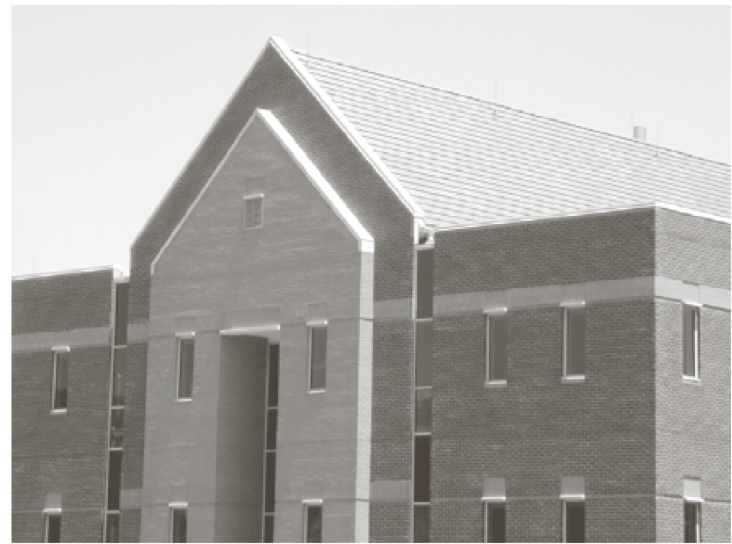
\includegraphics[height=7cm]{log_edge_original.png}
		\caption{Original image}
	\end{figure}
	
}

\frame{
	\frametitle{Laplacian of Gaussian (LoG): Illustration}
	\selectlanguage{english}
	\begin{figure}[!h]
		\begin{tabular}{cc}
			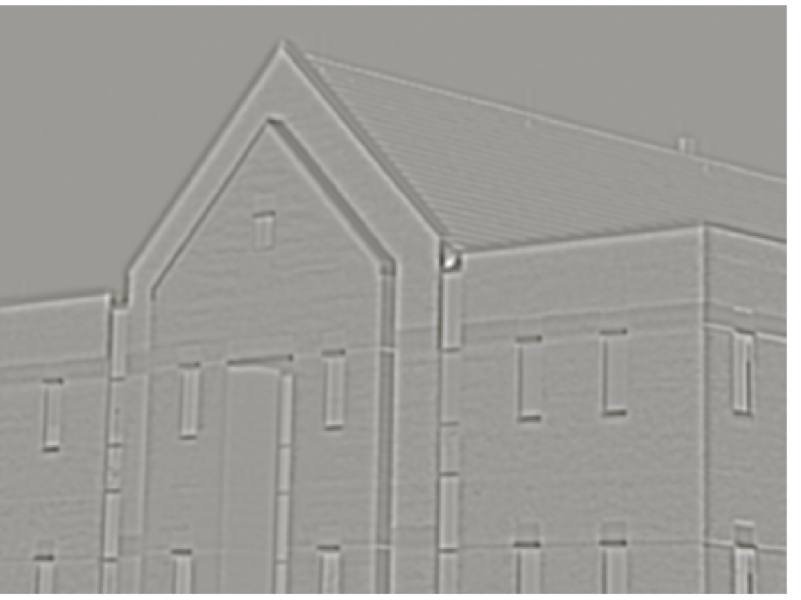
\includegraphics[width=4.5cm]{log_edge_step_1_2.png} &
			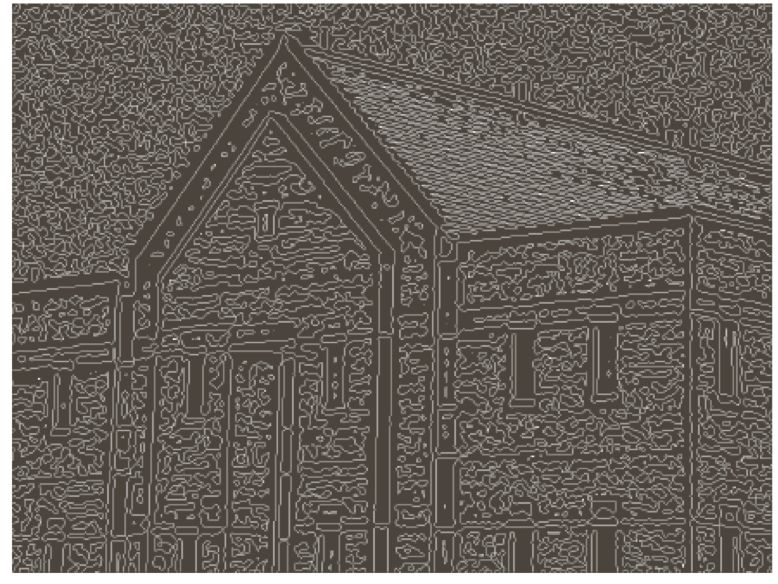
\includegraphics[width=4.5cm]{log_edge_zeros_cross_1.png}\\
			(a) & (b) \\
		\end{tabular}
		
		\caption{Marr-Hildreth Algorithm: (a): Result of Step $1$ and $2$, (b): Zero-crossing of (a), Threshold $=0$ }
	\end{figure}
	\begin{itemize}
		\item Step $1$ and $2$: $\sigma = 4, n = 25$ (kernel's size: $25 \times 25$) 
		\item Low threshold $\Rightarrow$ many edge points.
	\end{itemize}
	
}

\frame{
	\frametitle{Laplacian of Gaussian (LoG): Illustration}
	\selectlanguage{english}
	\begin{figure}[!h]
		\begin{tabular}{cc}
			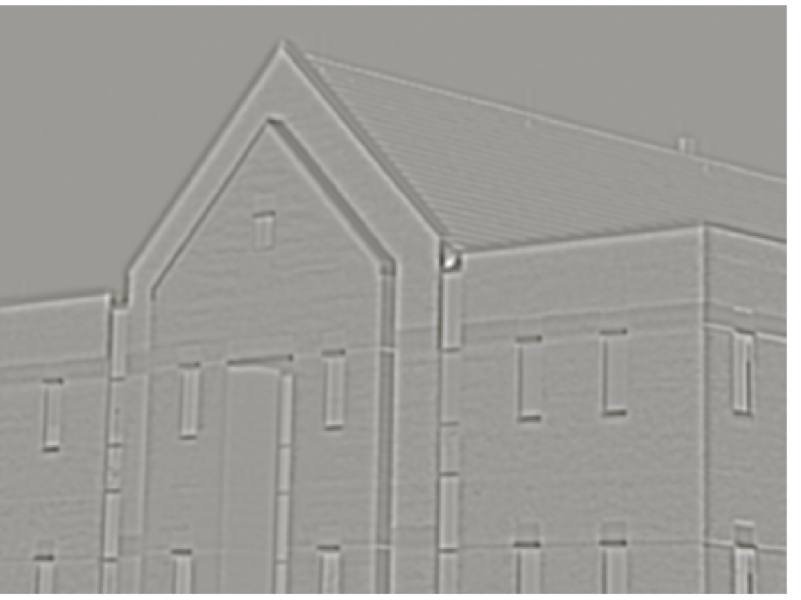
\includegraphics[width=4.5cm]{log_edge_step_1_2.png} &
			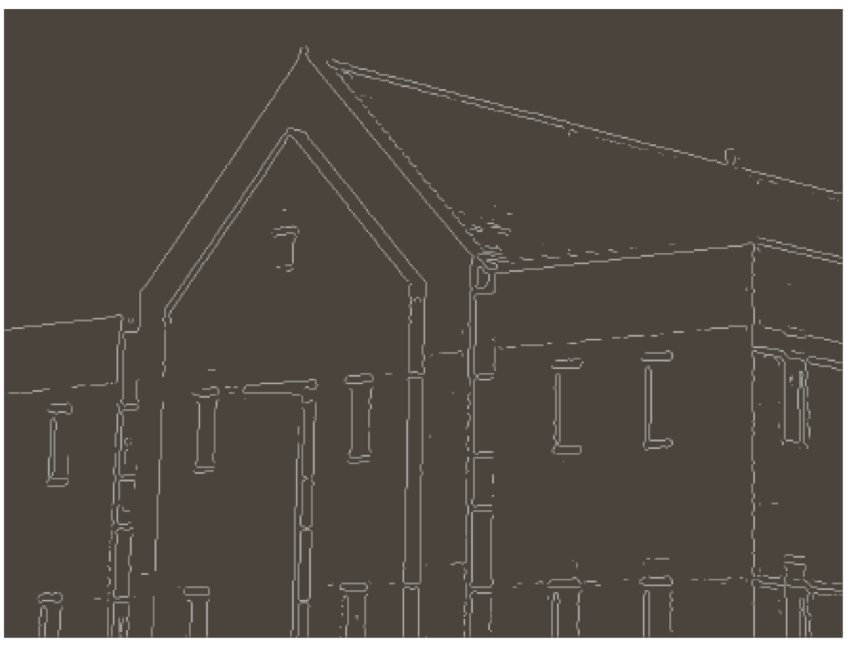
\includegraphics[width=4.5cm]{log_edge_zeros_cross_2.png}\\
			(a) & (b) \\
		\end{tabular}
		
		\caption{Marr-Hildreth Algorithm: (a): Result of Step $1$ and $2$, (b): Zero-crossing of (a), Threshold $= 4\%$ of maximum value in (a) }
	\end{figure}
	\begin{itemize}
		\item Step $1$ and $2$: $\sigma = 4, n = 25$ (kernel's size: $25 \times 25$) 
		\item Larger threshold $\Rightarrow$ provide strong edge only
	\end{itemize}
	
}
\frame{
	\frametitle{Canny Edge Detection}
	\selectlanguage{english}
	
	\begin{block}{Canny Edge Detection Algorithm}
		\begin{enumerate}
			\item Smooth the input image with Gaussian low-pass filter
			\item Compute the gradient magnitude angle images
			\item Apply nonmaxima suppression to the gradient magnitude image.
			\item Use double thresholding and connectivity analysis to detect and link edges
		\end{enumerate}
	\end{block}
	
}

\frame{
	\frametitle{Canny Edge Detection}
	\selectlanguage{english}
	
	\begin{block}{Step 1: Smooth the input image with Gaussian low-pass filter}
		\begin{enumerate}
			\item Smooth the input image with Gaussian low-pass filter
			\item Compute the gradient magnitude angle images
			\item Apply nonmaxima suppression to the gradient magnitude image.
			\item Use double thresholding to obtain strong and weak edge masks
			\item Analyze the connectivity to detect and link edges
		\end{enumerate}
	\end{block}
	
}
\frame{
	\frametitle{Canny Edge Detection}
	\selectlanguage{english}
	
	\begin{block}{Step 1: Smooth the input image with Gaussian low-pass filter}
	\end{block}
	
	\begin{align}
	\nonumber
	G(x,y) &= e^{-\frac{x^2 + y^2}{2\sigma^2}}\\
	\nonumber
	f_s(x,y) & = f(x,y) * G(x,y)
	\end{align}
	
	\begin{itemize}
		\item $f_s(x,y)$ : a smoothed version of $f(x,y)$
		\item $\sigma$ : decides the degree of smoothing
		\item $f_s(x,y)$ : Gaussian noise has been removed
	\end{itemize}
}
\frame{
	\frametitle{Canny Edge Detection}
	\selectlanguage{english}
	
	\begin{block}{Step 2: Compute the gradient magnitude angle images}
	\end{block}
		\begin{itemize}
			\item Compute $g_x(x,y)$ and $g_y(x,y)$
			\begin{equation}
			\begin{split}
				\nonumber
				g_x(x,y) & = f_s(x,y) * H_x(x,y)\\
				\nonumber
				g_y(x,y) & = f_s(x,y) * H_y(x,y)\\
			\end{split}
			\end{equation}
			\begin{itemize}
				\item $H_x(x,y)$, $H_y(x,y)$: any first-order derivative kernels, e.g., "standard" approximations kernels, Sobel, Roberts, Prewitts, etc.
			\end{itemize}
			\item Compute gradient magnitude and angle images
		\end{itemize}
		\begin{equation}
			\begin{split}		
				\nonumber
				M(x,y)  = \left[\begin{array}{c}
				g_x(x,y) \\
				g_y(x,y)
				\end{array}\right]\\
				\nonumber
				\alpha(x,y)  = tan^{-1}\left[ \frac{g_y(x,y)}{g_x(x,y)}\right]
			\end{split}
		\end{equation}
}
\frame{
	\frametitle{Canny Edge Detection}
	\selectlanguage{english}
	
	\begin{block}{Step 3: Apply nonmaxima suppression to the gradient magnitude image.}
	\end{block}
	\begin{block}{The underlying idea of \alert{\textbf{nonmaxima suprression}}}
		if a point is not a local maxima, then supress (remove, stop, etc) it.
	\end{block}
	\begin{itemize}
		\item Edges will pass points that are \alert{\textbf{local maxima}} in gradient magnitude image, ie., $M(x,y)$.
		\item $\Rightarrow$ Remove (supress) points that are not local maxima.
		\item $\equiv$ \alert{\textbf{nonmaxima suprression}}
	\end{itemize}
		
}
\frame{
	\frametitle{Canny Edge Detection}
	\selectlanguage{english}
	
	\begin{block}{Step 3: Apply nonmaxima suppression to the gradient magnitude image.}
	\end{block}
	\begin{block}{Questions}
		What does \alert{\textbf{local}} mean?
	\end{block}
	\begin{itemize}
		\item \alert{\textbf{local}} $\equiv$ local points involving in edge.
		\item for a point $(x,y)$ in $M(x,y)$, \alert{\textbf{which neighbor points are edge local points?}}
		\item $\Rightarrow$ need gradient angle
	\end{itemize}
	
	\begin{alertblock}{}
		Gradient vector at a point is \alert{\textbf{perpendicular}} to local edge at that point.
	\end{alertblock}
}
\frame{
	\frametitle{Canny Edge Detection}
	\selectlanguage{english}
	
	\begin{block}{Step 3: Apply nonmaxima suppression to the gradient magnitude image.}
	\end{block}
	\begin{enumerate}
		\item Discrete gradient angle values into small rangles.
		\item Find direction $d_k$ that is closest to $\alpha(x,y)$
		\item Find local neighbors on edge using $d_k$, referred to as $N_1$ and $N_2$
		\item Compute nonmaxima suppressed image $g_N(x,y)$
	\end{enumerate}
	\begin{equation}
		\begin{split}
			\nonumber
			g_N(x,y) =
			\begin{cases}
				0 & \text{if } \left[M(x,y) < N_1\right] \& \left[M(x,y) < N_2\right] \\
				M(x,y)& \text{otherwise}
			\end{cases}
		\end{split}
	\end{equation}
}

\frame{
	\frametitle{Canny Edge Detection}
	\selectlanguage{english}
	\begin{block}{Step 3: Apply nonmaxima suppression to the gradient magnitude image.}
	\end{block}
	\begin{figure}[!h]
		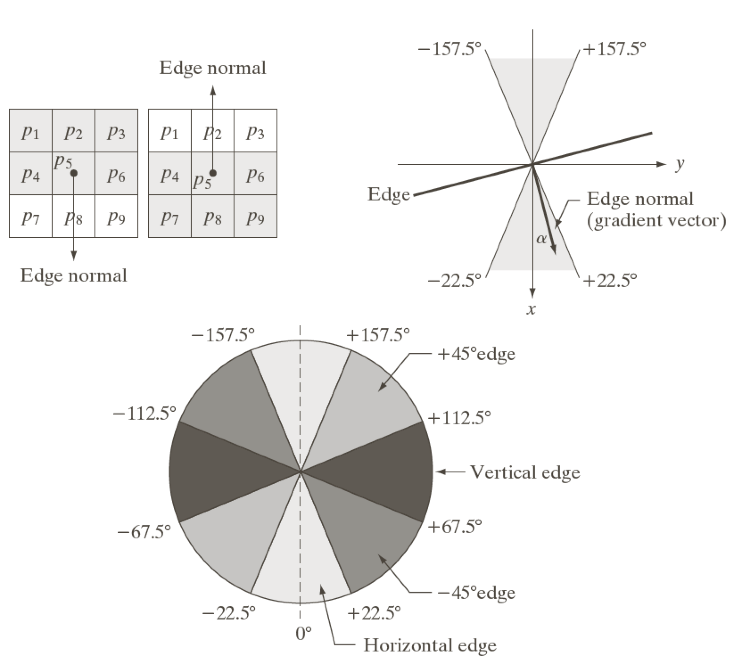
\includegraphics[height=6cm]{nonmaxima.png}
		\caption{Demonstration for 4 directions: horizontal, vertical, $\pm 45^0$}
	\end{figure}	
}
\frame{
	\frametitle{Canny Edge Detection}
	\selectlanguage{english}
	\begin{block}{Step 4: Use double thresholding to obtain strong and weak edge masks}
	\end{block}
	\begin{enumerate}
		\item Do thresholding with high and low threshold value $T_H$ and $T_L$ respectively.
		\begin{equation}
			\begin{split}
				\nonumber
				g_{NH}(x,y) &= g_N(x,y) \ge T_H\\
				g_{NL}(x,y) &= g_N(x,y) \ge T_L
			\end{split}
		\end{equation}
		
		\item Eliminate points in $g_{NL}(x,y)$ that has been indicated in $g_{NH(x,y)}$
			\begin{equation}
			\begin{split}
			\nonumber
				g_{NL}(x,y) &= g_{NL}(x,y) - g_{NH}(x,y)
			\end{split}
			\end{equation}
			
			\begin{itemize}
				\item 	$g_{NH}(x,y)$: strong edge
				\item 	$g_{NL}(x,y)$: weak edge
			\end{itemize}
			
	\end{enumerate}	
}
\frame{
	\frametitle{Canny Edge Detection}
	\selectlanguage{english}
	\begin{block}{Step 5: Analyze connectivity and to detect and link edges}
	\end{block}
	\begin{enumerate}
		\item Create an \alert{\textbf{edge map}} that marks all non-zeros in $g_{NH}(x,y)$ as valid edge points.
		\item For each pixel $p$ that is non-zeros in $g_{NH}(x,y)$, do
		\begin{itemize}
			\item Find all non-zeros pixels in $g_{NL}(x,y)$ that are connected to $p$ via $4-$ or $8-$connectivity, mark corresponding points in \alert{\textbf{edge map}} as valid pixels.
		\end{itemize}
	\end{enumerate}
	\begin{alertblock}{}
		\begin{itemize}
			\item \alert{\textbf{edge map}}  may contain edges thicker than 1 pixel.
			
			\item Apply edge-thinning algorithm to create thinner edge map, if needed.
		\end{itemize}
		
	\end{alertblock}
	
}


\frame{
	\frametitle{Canny Edge Detection: Illustration}
	\selectlanguage{english}
	\begin{figure}[!h]
		\begin{tabular}{cc}
			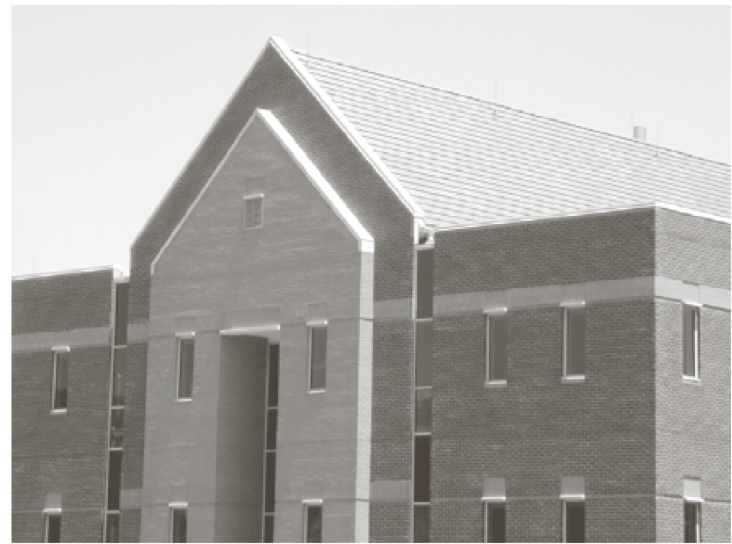
\includegraphics[width=4.5cm]{log_edge_original.png} &
			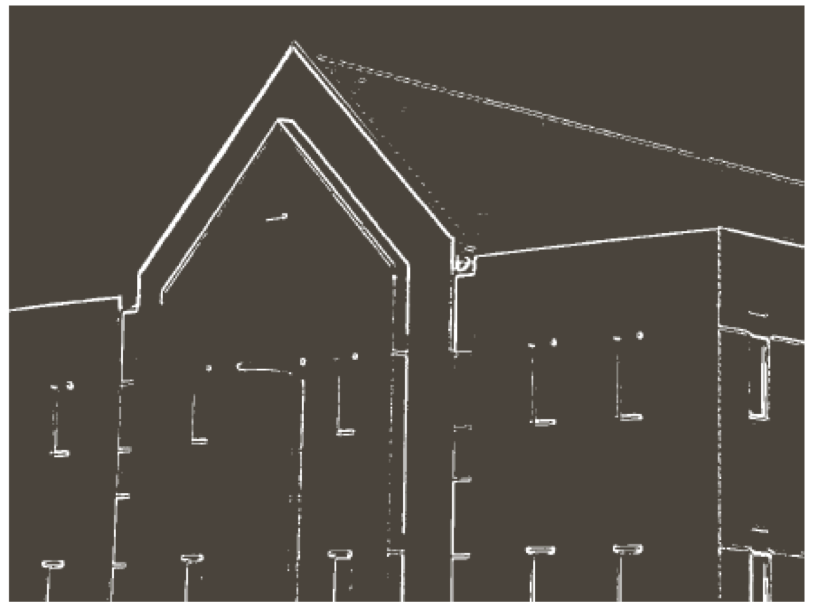
\includegraphics[width=4.5cm]{canny_edge_gradient.png}\\
			(a) & (b) \\
		\end{tabular}
		
		\caption{Edge detection (a): Original image, (b): Thresholded gradient magnitude image - \alert{\textbf{thick edge}}}
	\end{figure}
}
\frame{
	\frametitle{Canny Edge Detection: Illustration}
	\selectlanguage{english}
	\begin{figure}[!h]
		\begin{tabular}{cc}
			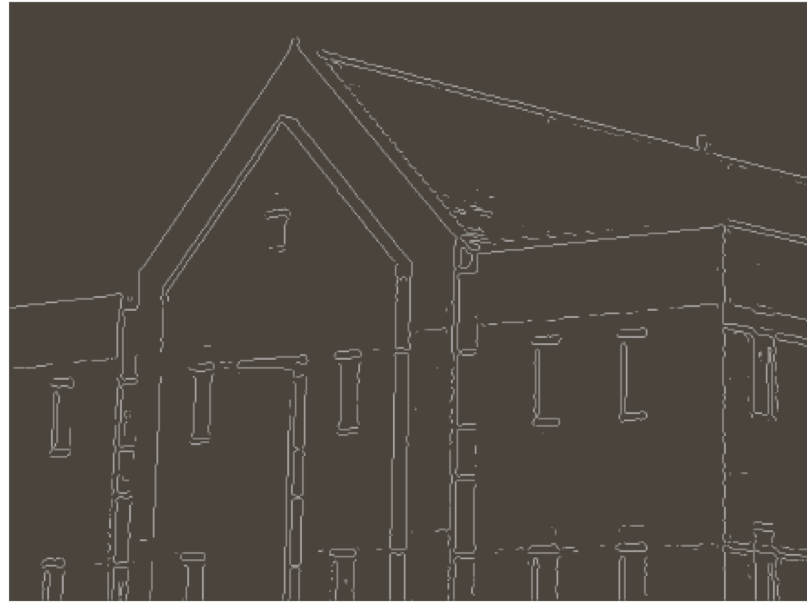
\includegraphics[width=4.5cm]{canny_edge_log.png} &
			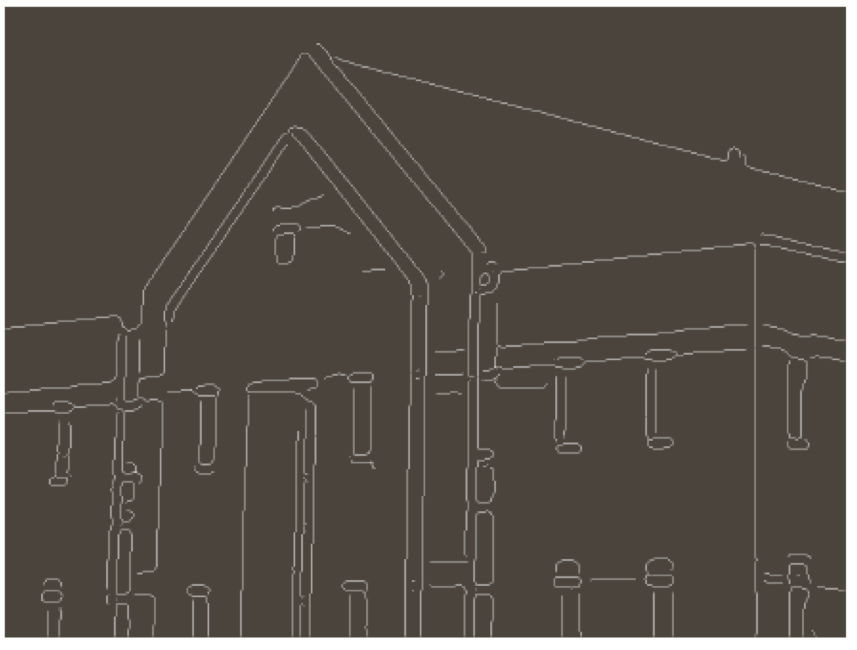
\includegraphics[width=4.5cm]{canny_edge_canny.png}\\
			(a) & (b) \\
		\end{tabular}
		
		\caption{Edge detection (a): Marr-Hildreth Method, (b): Canny method - \alert{\textbf{better}}}
	\end{figure}
}
%%%%%%%%%%%%%%%%%%%%%%%%%%%%%%%%%%%%%%%%%%%%%%%

%%%%%%%%%%%%%%%%%%%%%%%%%%%%%%%%%%%%%%%%%%%%%%%

\end{document}